\documentclass[a4paper, 12pt]{article}
\usepackage[left=2.5cm, right=2.5cm, top=3cm, bottom=3cm]{geometry}
\usepackage[spanish]{babel}
\usepackage{amsmath}
\usepackage{graphicx}
\usepackage{color}
\usepackage{xcolor}
\usepackage[utf8]{inputenc}
\usepackage[T1]{fontenc}
\usepackage{listings}
\usepackage{tikz}
\usetikzlibrary{shapes,arrows,positioning}




\definecolor{colorgreen}{rgb}{0,0.6,0}
\definecolor{colorgray}{rgb}{0.5,0.5,0.5}
\definecolor{colorpurple}{rgb}{0.58,0,0.82}
\definecolor{colorback}{RGB}{255,255,204}
\definecolor{colorbackground}{RGB}{211,211,211}
%Definiendo el estilo de las porciones de codigo
\lstset{
 backgroundcolor=\color{colorbackground},
commentstyle=\color{colorgreen},
keywordstyle=\color{colorpurple},
numberstyle=\tiny\color{colorgray},
stringstyle=\color{colorgreen},
basicstyle=\ttfamily\footnotesize,
breakatwhitespace=false,
breaklines=true,
captionpos=b,
keepspaces=true,
numbers=left,
showspaces=false,
showstringspaces=false,
showtabs=false,
tabsize=2,
frame=single,
framesep=2pt,
rulecolor=\color{black},
framerule=1pt
}



\begin{document}


\begin{center}
\text{\Huge GEOWALL- E}\\
\vspace {2cm}
\text{\huge Mauricio Sunde Jiménez C111}\\
\vspace {0.5cm}
\text{\huge Richard Alejandro Matos Arderí C111}\\
\vspace {0.5cm}
\text{\Large Facultad de Matemática y Computación, Universidad de La Habana}\\
\vspace {0.5cm}
\text{2023}\\
\vspace {10cm}
\begin{figure}[h]
       \center
       
\includegraphics[width=8cm]{matcom.jpg}
\end{figure}
\end{center}

\newpage
\begin{abstract}
GEOWALL- E es una aplicación capaz de representar conceptos geométricos, como puntos, líneas o circunferencias, graficarlos y comprobar  que relaciones básicas conocidas de la geometía se cumplen.
\end{abstract}
\tableofcontents
\newpage

\section{Introducción}\label{sec;intro}



\newpage
\section{¿Cómo usarlo?}

Una vez ejecutado el proyecto desde la carpeta raíz, el usuario será direccionado a la interfaz gráfica diseñada sobre la plataforma Windows Form. En la interfaz encontrará un cuadro de texto capaz de recepcionar el código de G \# , y una vez presionado el botón ´DRAW´  aparecerá en pantalla, específicamente en la región del lienzo la representación geométrica (en caso de que el código la tuviese) , de lo introducido por el usuario.
Ejemplo:
\begin{figure}[h]
       \center
       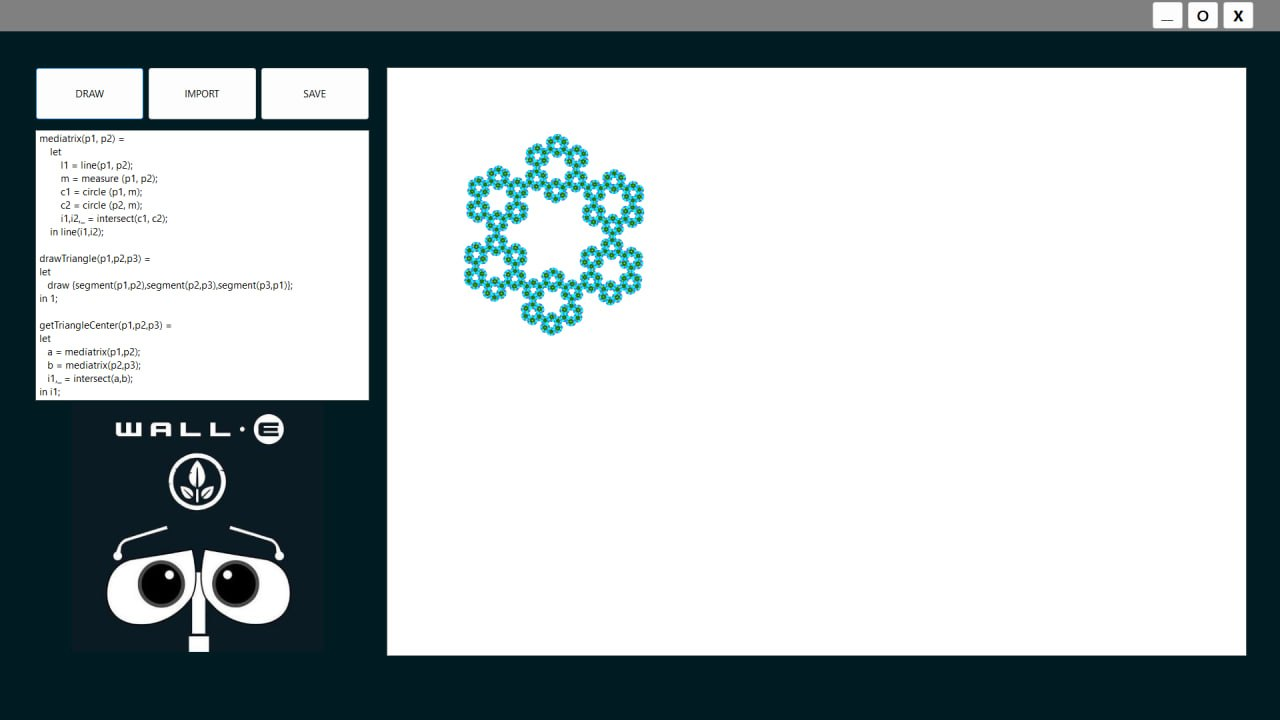
\includegraphics[width=8cm]{nieve.jpg}
\end{figure}

Otras funcionalidades están sobre los botones ´IMPORT´ y ´SAVE´.
 La ejecución del primero se basa en llamar al Administradorde archivos prederteminado del sistema , para seleccionar un archivo que contenga un código en G \# que se desea representar. Una vez seleccionado el texto que contiene aparecerá automáticamente en el cuadro de texto de la interfaz , listo para ser procesado.
El botón ´SAVE´ de forma análoga al anterior llama al  Administradorde archivos prederteminado del sistema , pero con el objetivo opuesto, en lugar de importar información , se busca guardar en un archivo compatible, el código que se encuentra sobre el cuadro de texto en el momento de la ejecución de esta funcionalidad.
 Ejemplo:
\begin{figure}[h]
       \center
       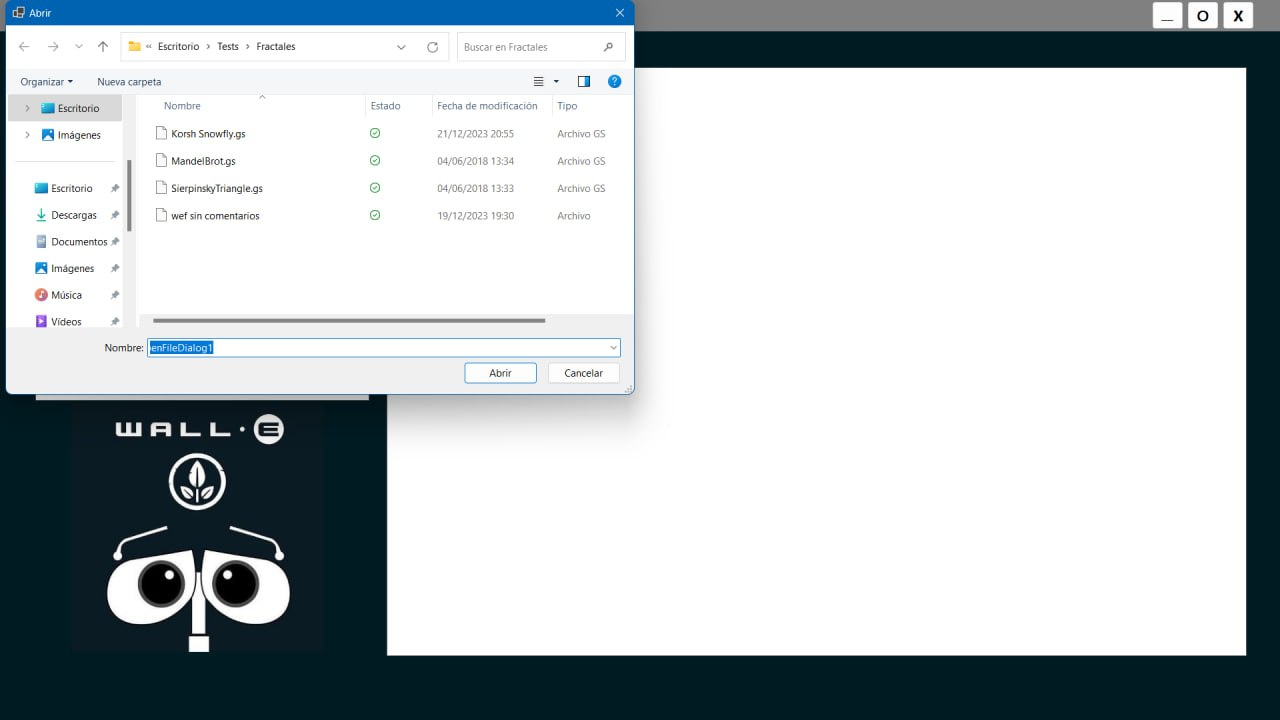
\includegraphics[width=8cm]{import.jpg}
\end{figure}

   


\paragraph{\textcolor{blue}{De forma general solo serán representadas en el lienzo instrucciones que constituyan declaraciones de tipo \textcolor{red}{draw}  válidas.}}



\newpage
\section{Estructura del proyecto}\label{}


\subsection{Interfaz Gráfica}\label{}
La interfaz gráfica está implementada sobre Windows Form.

El formulario principal es construido cuando se ejecuta el proyecto (el flujo de ejcución comienza con el método Main de la clase Program, aquí se inicializa el formulario cuyo código funcional recae en la clase GEOWALL- E). Esta clase contiene los métodos que responden ante el uso de los botones implementados. El principal sería el método DRAWCLICK, quien dirige todos los procesos de procesamiento de la entrada del usuario (dígase parsing, chequeo de tipos y evaluación). A cotinuación el siguiente listado ilustra el código del método:

\begin{lstlisting}[language= Java]
private void DRAWClick(object sender, EventArgs h)
{
            Papel.Clear(BackColor);
            Papel.Clear(ForeColor);
            string Entrada = PANELCOMANDOS.Text;
            if (Entrada != string.Empty)
            {
                try
                {
                    StandardLibrary.Initialize(); 
                    WallEColors.InitializeColor();
                    var statements = StatementsTree.Create(Entrada);
                    TypeChecker.CheckType(statements);
                    GSharpEvaluator evaluator = new(statements);
                    var result = evaluator.Evaluate();
                }
                catch (Exception e)
                {
                    MessageBox.Show(e.Message);
                }
            }
 }
\end{lstlisting}


\subsubsection{Uso de System.Drawing: \textcolor{cyan}{Clase graphics}}\label{}
La clase Graphics en C\# es parte del espacio de nombres System.Drawing y proporciona funcionalidades para dibujar gráficos en una superficie, como un formulario o un control. Se utiliza para realizar operaciones de dibujo, como trazar líneas, dibujar formas, texto, imágenes, etc.  Proporciona métodos para dibujar y rellenar formas geométricas, trabajar con colores, fuentes, transformaciones, entre otros que fueron empleados para cubrir estas funcionalidades en GEOWALLE-E. A continuación se listan los métodos principales que fueron empleados:

\begin{itemize}
\item \textcolor{magenta}{DrawEllipse}: Este método dibuja una elipse delimitada por un rectángulo especificado. Se utiliza para dibujar el contorno de una elipse. Fue adpatado para dibujar circunferencias, como caso particular de una elipse delimitada por un cuadrado cuya longitud de lado coincide con el diámetro de la circunferencia en cuestión.

\item \textcolor{magenta}{ DrawArc}: Dibuja un arco delimitado por un rectángulo especificado. Puede ser utilizado para dibujar una porción de una elipse o círculo. Fue utilizado para dibujar el objeto \textcolor{cyan}{Arc} ,propio de la biblioteca \textcolor{blue}{GSharpProject}, que representa un arco de circunferencia.

\item \textcolor{magenta}{ FillEllipse}: Rellena el interior de una elipse delimitada por un rectángulo especificado con un color sólido. Fue empleado para representar en el lienzo al objeto  \textcolor{cyan}{Point}, propio de la biblioteca \textcolor{blue}{GSharpProject}, que representa un punto.

\item \textcolor{magenta}{ DrawLine}: Dibuja una línea entre dos puntos especificados. Este método fue empleado para representar los objetos de la biblioteca \textcolor{blue}{GSharpProject} : \textcolor{cyan}{Line}, \textcolor{cyan}{Segment} y \textcolor{cyan}{Ray} que represenntan respectivamente una línea, un segmento y un rayo(entiéndase por esto una recta con un extremo).
\end{itemize}
\subsubsection{Diseño}\label{}
El diseño recae en el archivo archivo ´Form1.Designer.cs´ que es generado por Visual Studio para definir y configurar los controles y componentes de un formulario de Windows Forms. 

Algunos aspectos clave son:
\begin{itemize}
\item \textit{Configuración de Controles}: Establece las propiedades y disposiciones de los controles visuales en el formulario, como botones, etiquetas, paneles y cuadros de texto. Por ejemplo, se agregan controles como 'PANEL\_DIBUJO', 'DRAW', 'IMPORT', 'CLOSE\_BTN', 'MIN\_BTN', 'MAX\_BTN', entre otros, y se definen algunas de sus propiedades como color, ubicación y tamaño.

\item \textit{Configuración de Formulario}: Define las propiedades y comportamiento del formulario en sí, como su tamaño, color de fondo, nombre, eventos asociados, etc. Esto incluye el manejo de eventos como 'Load' y 'MouseDown'.

\item \textit{Ajustes de Visualización}: El código incluye ajustes de diseño y visualización, como el anclaje y el escalado de los controles para que se adapten y se muestren correctamente en el formulario.
\end{itemize}

\newpage
\subsection{Intérprete de G\#}\label{}
El intérprete de G\# implementado responde al procesamiento de una cadena de texto apoyado en tres fases principales: parsing(análisis sintáctico) , chequeo de tipos y evaluación.
\subsubsection{Parsing}\label{}
El método Parse es llamado desde  el método de tipo GharpStatementsCollection, Create perteneciente a la clase StatementsTree , invocado en DRAWClick. Con esta llamada se tokeniza la cadena de caracteres (string) introducida por el usuario, esta tokenización se realiza en el constructor de la clase Parser y se apoya en la clase Lexer y us métodos de reconocimiento de tokens. El parsing se basa en construir objetos del árbol de expresiones de GSharpProject , cuya jerarquía de herencia es ilustrada en el siguiente esquema:
\begin{tikzpicture}[
level distance=6cm,
  grow=right,
  level 1/.style={sibling distance=1cm},
  level 2/.style={sibling distance=1cm},
  level 3/.style={sibling distance=1cm},
 every node/.style = {shape=rectangle, rounded corners,
      draw, align=center}
]

  
  % Nodos
  \node[rectangle, draw, fill=blue!20] (A) at (0,0) {GSharpExpression}
    
    child {
      node[rectangle, draw, fill=red!20] (B) {AssignmentExpression}}
    child {
      node[rectangle, draw, fill=red!20] (C) {ColorExpression}}
    child {
      node[rectangle, draw, fill=red!20] (D) {DrawExpression}}
    child {
      node[rectangle, draw, fill=red!20] (E) {FunctionCallExpression}}
     child {
      node[rectangle, draw, fill=red!20] (F) {FunctionDeclarationExpression}}
     child {
      node[rectangle, draw, fill=red!20] (I) {GSharpPrimitive}
               child {
               node[rectangle, draw, fill=green!20] (J) {GSharpLiteralExpression}}
               child {
               node[rectangle, draw, fill=green!20] (K) {GSharpPointExpression}}
             child {
               node[rectangle, draw, fill=green!20] (L) {GSharpRayExpression}}
                child {
               node[rectangle, draw, fill=green!20] (M) {GSharpSegmentExpression}}
              child {
               node[rectangle, draw, fill=green!20] (N) {GSharpCircleExpression}}
                child {
               node[rectangle, draw, fill=green!20] (O) {GSharpLineExpression}}
             child {
               node[rectangle, draw, fill=green!20] (P) {GSharpArcExpression}}}
    child {
      node[rectangle, draw, fill=red!20] (G) {FunctionReference}}
     child {
      node[rectangle, draw, fill=red!20] (H) {GSharpBinaryExpression}}
      child {
      node[rectangle, draw, fill=red!20] (U) {GSharpUnaryExpression}}
     child {
      node[rectangle, draw, fill=red!20] (V) {GSharpVoidEx}}
      child {
      node[rectangle, draw, fill=red!20] (W) {If\_ElseStatement}}
     child {
      node[rectangle, draw, fill=red!20] (X) {Let\_In\_Expression}}
      child {
      node[rectangle, draw, fill=red!20] (Y) {MeasureExpression}}
     child {
      node[rectangle, draw, fill=red!20] (Z) {SequenceOf}}
  child {
              node[rectangle, draw, fill=red!20] (Q) {GSharpSequence}
                child {
                node[rectangle, draw, fill=green!20] (R) {GSharpInfiniteSequence}}
                child {
                node[rectangle, draw, fill=green!20] (S) {GSharpRangeSequence}}
                child {
                node[rectangle, draw, fill=green!20] (T) {GSharpLiteralSequence}}}
    child {
      node[rectangle, draw, fill=red!20] (AB) {GSharpStatementsCollection}};

\end{tikzpicture}
\newpage
\subsubsection{Chequeo de tipos}\label{}
Cada una de las clases del árbol de expresiones contiene el método void CheckType, pues la clase abstracta GSharpExpression lo contiene como método abstracta. De esto se deduce que cada nodo sepa \" chequear su tipo \" . En caso de alguna inconsistencia con las condiciones de validez de una expresión determinada , la ejecución de este método ,llamado desde el método DRAWClick y aplicado sobre cada una de las expresiones resultado del parsing , nos alertará del error y se detendrá el procesamiento de la entrada actual. Como asistente esencial de este proceso está la clase \textit{static} \textcolor{blue}{ TypeCheckerHelper} que contiene un diccionario
\textcolor{magenta}{binaryTypesDic} que contiene los patrones de tipo válidos para expresiones de G\#.
 
\subsubsection{Evaluación: Clase GSharpEvaluator}\label{}
La evaluación en GEOWALL-E se realiza gracias a la clase \textcolor{blue}{ GSharpEvaluator} que recibe un nodo GSharpStatementsCollection ya una vez chequeado su tipo. Cuando en la clase GEOWALL\_E se instancia este objeto , seguido se llama al método Evaluate que por cada declaración en la propiedad \_Nodo la clasifica y de acuerdo a su tipo la redirecciona al método de evaluación correspondiente. De manera particular si se trata de una expresión DrawExpression son es llamado el método void Draw de la clase GEOWALL-E encargado de representar el objeto dibujable en el lienzo, de lo contrario los métodos se restringen a retornar el valor de retorno (en caso de existir) de la expresión evaluada.

\subsubsection{Geometría}\label{}
Los objetos geométricos implementados en la biblioteca GSharpProject implementan la interfaz IFigure, cuyo código se representa en el siguiente listado:

\begin{lstlisting}[language= Java]
 public interface IFigure
{
        bool PointBelong(Point p1);
        IEnumerable<Point> PointsOf();
}
\end{lstlisting}
Esta interfaz nos permite aprovechar las funcionalidades de saber si un punto pertenece o no a un objeto geométrico determinado y obtener un \textcolor{magenta}{\texttt{IEnumerable<\textcolor{cyan}{Point}>}} que nos brinda la posibilidad de acceder a inifinitos puntos de un objeto.
Los objetos geométricos implementados son:
\begin{itemize}
\item \textcolor{cyan}{Point}: Punto determinado por un par ordenado de valores double.
\item \textcolor{cyan}{Line}: Recta determinada por dos puntos.
\item \textcolor{cyan}{Segment}: Segmento determinado por dos puntos.
\item \textcolor{cyan}{Ray}: Línea determinada por un punto de inicio y otro punto que marca la dirección sobre la que la línea es infinita.
\item \textcolor{cyan}{Arc}: Arco determinado por un punto centro, una medida de radio, y dos puntos (los rayos determinados por cada uno y el centro que determinan el ángulo que cubre el arco).
\item  \textcolor{cyan}{Circle}: Circunferencia determinada por un punto centro y una medida de su radio.
\end{itemize}

Sobre conceptos geométricos es esencial también la clase  \textcolor{blue}{Utiles}, que contiene métodos static que brindan funciones de la Geometría Analítica tales como la Distancia Euclidiana entre dos puntos y el conjunto intersección de dos lugares geométricos.

\section{Conclusiones}\label{sec:concl}
La creación de este proyecto ha sido sumamente instructiva sobre temas como encapsulamiento, modularización, herencia, y polimorfismo por lo que  ha contribuido sólidamente a fortalecer habilidades como la investigación y otras menos interactivas pero igualmente importantes como son la organización y la planificación, tan necesarias para la vida profesional.
\end{document}












































